\chapter{Grundlagen}
Dieses Kapitel verschafft einen Überblick über die benötigten theoretische Grundlagen, um die Methoden dieser Arbeit zu verstehen. Als
erstes wird der ``Lab-Farbraum'' kurz erklärt. Als nächstes wird eine Einführung in Neuronale Netzwerke gegeben, anschließend werden
einzelne Bestandsteile und Varianten von Neuronalen Netzwerken erklärt. Abschließend wird einen Überblick über verwandte Arbeiten gegeben.

\section{\textit{Lab}-Farbraum} 
Der \textit{Lab}-Farbraum (auch CIELAB-Farbraum genannt) ist ein Farbraum definiert bei der Internationale
Beleuchtungskommission (\gls{cie}) in 1976. Farben werden mit drei Werte beschrieben. ``\textit{L}'' (Lightness) definiert die Helligkeit.
Die Werte liegen zwischen 0 und 100. ``\textit{a}'' gibt die Farbart und Farbintensität zwischen Grün und Rot und ``\textit{b}'' gibt die
Farbart und Farbintensität zwischen Blau und Gelb. Die Werte für ``\textit{a}'' und ``\textit{b}'' liegen zwischen -128 und 127.

TODO: image
% TODO: add color space image
% \begin{figure}[H]
%   \centering
%   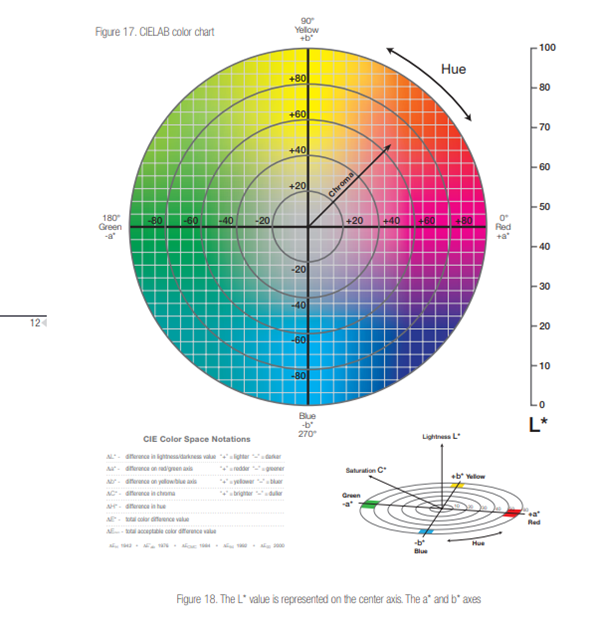
\includegraphics[width=0.5\textwidth]{resources/colorspace/lab-color-space.png}
%   \caption{CIELAB Farbraum}
%   \label{}
% \end{figure}

\section{Neuronale Netze}
Künstliche Neuronale Netze sind inspiriert durch das Menschliche Gehirn und werden für Künstliche Intelligenz und Maschinelles Lernen
angewendet. Neuronale Netze bestehen aus Neuronen oder auch ``Units'' genannt, die Schichtenweise in ``Layers'' (Schichten) angeordnet sind.
\\
\\
Beginnend mit der Eingabeschicht (Input Layer) fließen Informationen über eine oder mehrere Zwischenschichten (Hidden Layer) bis hin zur 
Ausgabeschicht (Output Layer). Dabei ist der Output des einen Neurons der Input des nächsten. \cite{neuronale-netze-aufbau}

\subsection{Feedforward Neuronal Network}
Das Ziel von einem Feedforward Neuronal Network ist die Annäherung an irgendeine Funktion $ f^* $. Feedforward Neuronal Network definiert 
eine Abbildung $ y = f(x;\theta) $ wo $ x $ den Input ist und $ \theta $ die lernbare Parameter sind (auch weights genannt).
\cite[164-223]{Goodfellow-et-al-2016}
\\
\\
Diese Netzwerkarchitektur heißt ``feedforward'' weil der Informationsfluss von der Input Layer über die Hidden Layers bis zur Output Layer 
in einer Richtung weitergereicht wird.

\begin{figure}[H]
  \centering
  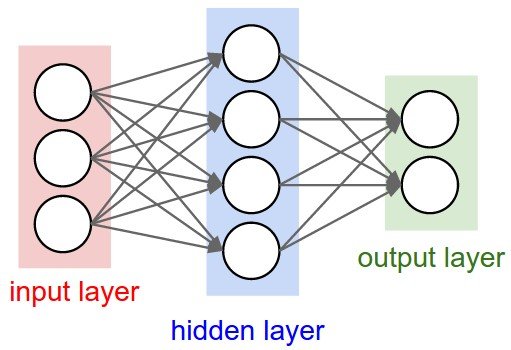
\includegraphics[width=0.65\textwidth]{resources/nn/neural_net.jpeg}
  \caption{
    Fully-connected Neuronal Network mit 2 Layers (ein Hidden Layer mit 4 Neuronen) und ein Output Layer mit 2 Neuronen 
    \cite{fully-connected-neural-network}
  }
  \label{image:neuronal-network}
\end{figure}

Feedforward Neuronal Network werden repräsentiert als eine Kette von Funktionen und daher werden sie Netzwerke genannt. Als Beispiel,
kann man die Funktionen $ f^{(1)}, f^{(2)}, f^{(3)} $ in Form einer Kette verbinden um $ f(\textbf{x}) = f^{(3)}(f^{(2)}(f^{(1)}(\textbf{x}))) $
zu bekommen. Diese Kettenstrukturen sind die am häufigsten genutzte Struktur bei Neuronale Netzwerke. In diesem Fall, $ f^{(1)} $ ist das 
erste Layer, $ f^{(2)} $ das zweite und $ f^{(3)} $ der Output Layer von diesem Netzwerk. Die Länge dieser Kette definiert die Tiefe von einem Netzwerk. Je tiefer
ein Netzwerk ist desto mehr lernbare Parameter hat es und somit eine erhöhte Rechenleistung braucht um trainiert zu werden.
In der Praxis werden die Netzwerke sehr tief, daher der Begriff Deep Learning.

\subsection{Fully-connected Neuronal Network}
\subsection{Aktivierungsfunktionen}
\subsection{Convolutional Neuronal Network}
\subsection{Andere Layers}
\subsection{Kostenfunktionen}
\subsection{Backpropagation}\label{subsection:backpropagation}
\subsection{Optimierungsalgorithmen}
% Beispiel Abbildung \ref{img:cnn_example_network} mit Zitat. \begin{figure}[H] \centering
% 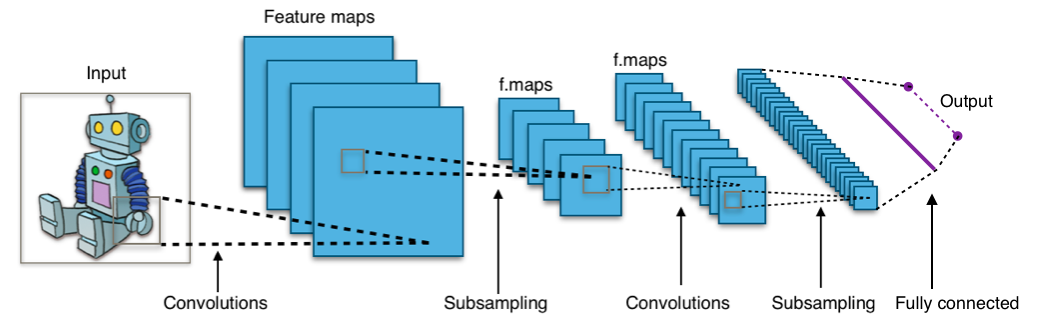
\includegraphics[width=0.95\textwidth]{resources/cnn/typical_cnn} \caption{Beispiel CNN Architektur \cite{typical_cnn_img}}
% \label{img:cnn_example_network} \end{figure}
\section{Verwandte Arbeiten}
TODO